
\chapter{Menu Landmarks}\label{landmark_chapter}
\minitoc 


As stated above, landmarks can be set on surfaces by pressing ``L" + left mouse click. Several actions
can be performed on landmarks.


\section{Select landmark range}
\noindent
\begin{minipage}{0.5\textwidth}
By opening the ``select landmark range" window, you can
select a given range of landmarks. This option may be useful
when you need to save only a specific sub-range of all digitized landmarks.
\end{minipage}    
\begin{minipage}{0.5\textwidth}\centering
  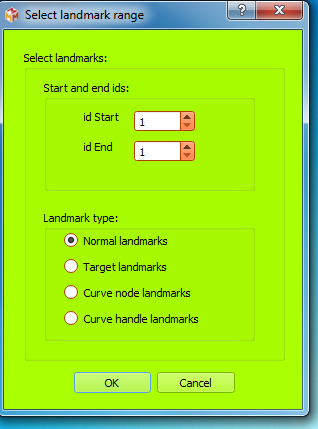
\includegraphics[scale=0.5]{images/10/select_landmark_range.png}
 \captionof{figure}{Select landmark range window}
 \end{minipage} 
\noindent


\section{Selected landmarks: decrease landmark number (move up in list)}
This option will increase (=move up in list, if possible) the landmark number of all selected landmarks. This option can be also activated by clicking on 
\includegraphics[scale=0.7]{images/06/objects/move_up.png} in the "object controls" section of the main window.
 
\section{Selected landmarks: increase landmark number (move down in list)}
 This option will decrease (=move down in list, if possible) the landmark number of all selected landmarks.
This option can be also activated by clicking on 
\includegraphics[scale=0.7]{images/06/objects/move_down.png} in the "object controls" section of the main window.

\section{Selected landmarks: push back on closest surface's vertex}
When set via pressing ``L" + left click, landmarks are always positioned at a surface's vertex coordinates. Selected
landmarks can be subsequently moved manually to other locations (for instance, if you want to place
a given landmark in the middle of a canal or of a foramen, or between two unfused bones). However,
you may sometimes want to push back automatically some selected landmarks to the position of the
closest surface's vertex available. This can be achieved using this option (see for instance Fig. \ref{push_back} p.\pageref{push_back}).

\begin{figure}
  \centering
  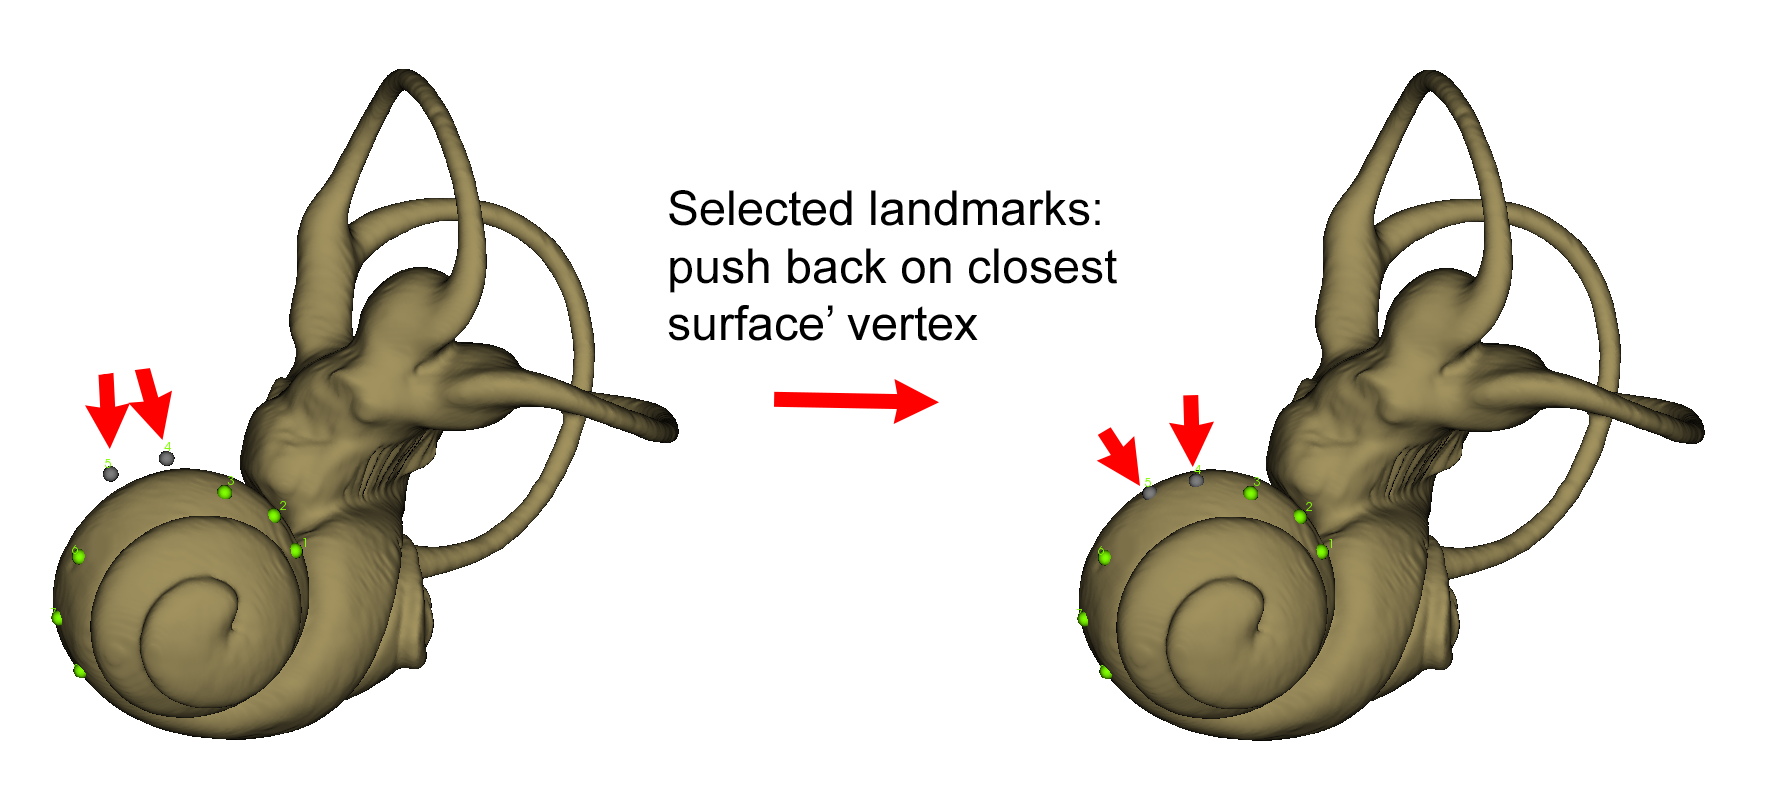
\includegraphics[scale=0.27]{images/10/push_back.png} 
	\caption{Push back selected landmarks on surface's closest vertex. A: two landmarks (4 and 5) laying outside the surface of the left inner of a \textit{Galago moholi} specimen have been selected. B: these 2 landmarks now lay on the surface. This action can be undone/redone.}
\label{push_back}
 
\end{figure}


\section{Selected landmarks: change orientation according to surface's normals}
When set via pressing ``L" + left surfaces, landmark orientation is that of the vertex on which it is
placed. Selected landmarks' orientation can be subsequently moved manually. However, you may
sometimes want to reset one or several landmarks' orientation automatically to that of the normal of the closest
surface's vertex available. This can be achieved using this option (see for instance Fig. \ref{reorient} p.\pageref{reorient}).

\begin{figure}
  \centering
  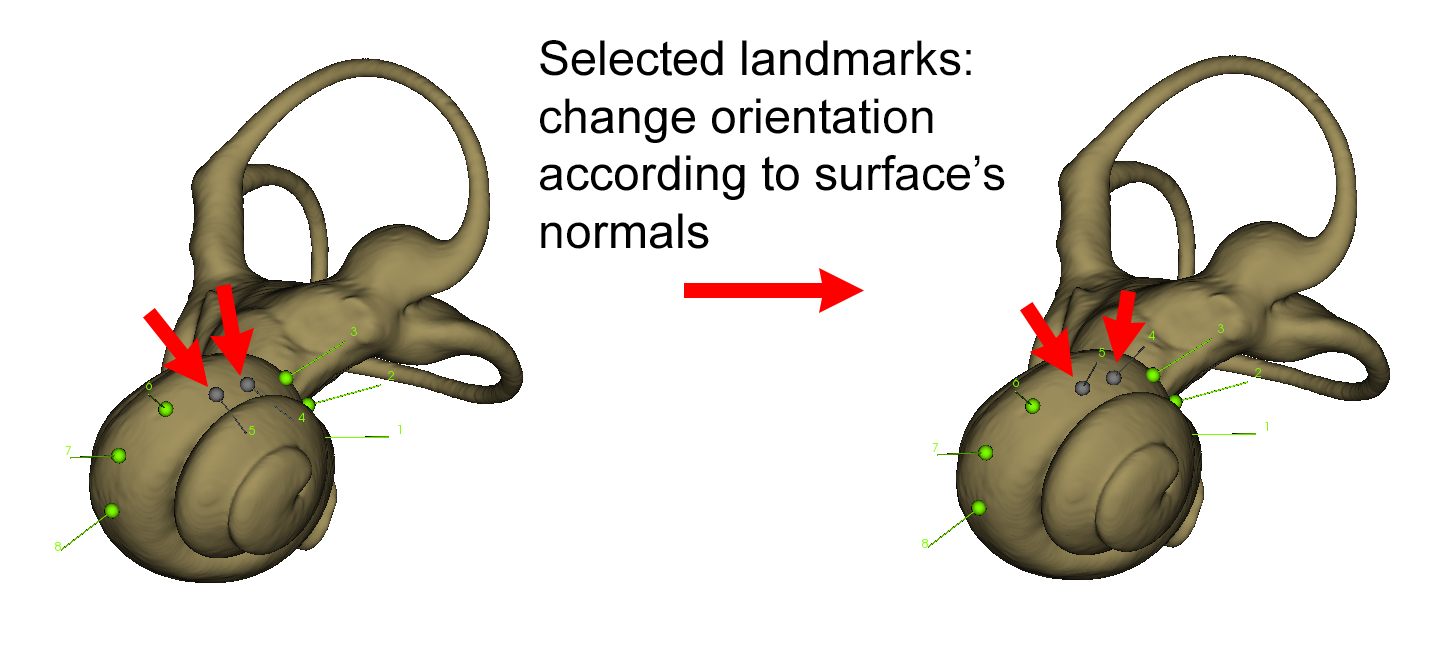
\includegraphics[scale=0.3]{images/10/reorient.png} 
	\caption{Change orientation according to surface's normals. A: two landmarks (4 and 5) the surface of the left inner of a \textit{Galago moholi} specimen have been selected. B: these 2 landmarks' orientation now is the same as that of the closest vertices. This action can be undone/redone.}
\label{reorient}
 
\end{figure}


\section{Selected curve nodes and curve handle landmarks}\label{landmarks_curves_section}
Before reading this paragraph, in order to get a good understanding  about how curves are constructed in MorphoDig, please make sure you have read carefully the section \ref{file_curve_section} p.\pageref{file_curve_section}.
\subsection{Move curve handles semi-automatically}
\noindent
\begin{minipage}{0.5\textwidth}
This option allows saving a lot of time when creating
3D Bezier curves with MorphoDig (see Fig. \ref{move_handles} p.\pageref{move_handles}). Also see ``working
with curves" tutorial for further details regarding curve digitization with MorphoDig).
\end{minipage}    
\begin{minipage}{0.5\textwidth}\centering
  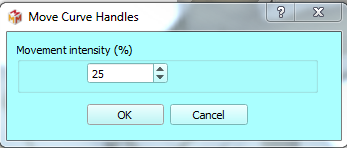
\includegraphics[scale=0.5]{images/10/move.png}
 \captionof{figure}{Mode handles window}
 \end{minipage} 
\noindent



Requirement : at least a handle landmark (``purple" landmark) must be selected.
Depending on whether selected curve handles lie within the curve, at the start of the curve or at the
end of the curve, their displacements differ (see Fig. \ref{move_handles2} p. \pageref{move_handles2})




\begin{figure}
  \centering
  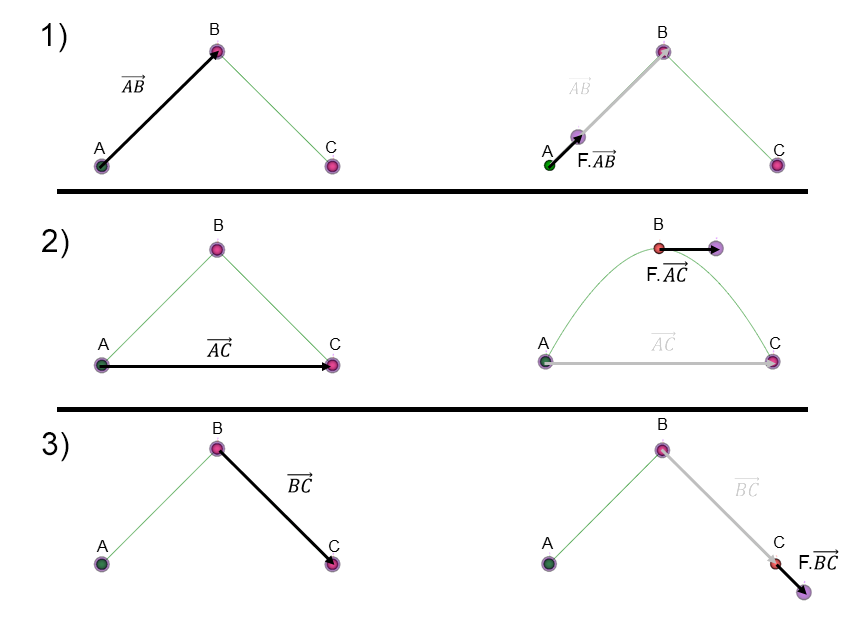
\includegraphics[scale=0.7]{images/10/fig_disp.png} 
	\caption{ Moving handles semi-automatically. \newline 1. Left: curve handle is associated to a curve starting point (A), and a following point (B) exists. Vector $\overrightarrow{AB}$ is computed, as well as its length |AB|. Right: curve handle associated to A is moved from point A along $\overrightarrow{AB}$. Displacement length=movement intensity/|AB|.\newline 2. Left: curve handle is associated to a point B lying between two points (A and C). Vector $\overrightarrow{AC}$ is computed, as well as its length |AC|. Right: curve handle associated to B is moved from point B along $\overrightarrow{AC}$. Right: displacement length=movement intensity/|AC|.  \newline 3. Left: curve handle is associated to a curve ending point (C), and a preceding point (B) exists. Vector $\overrightarrow{BC}$ is computed, as well as its length |BC|. Right: curve handle associated to C is moved from point C along $\overrightarrow{BC}$. Displacement length=movement intensity/|BC|. }
	
\label{move_handles}
 
\end{figure}

\begin{figure}
  \centering
  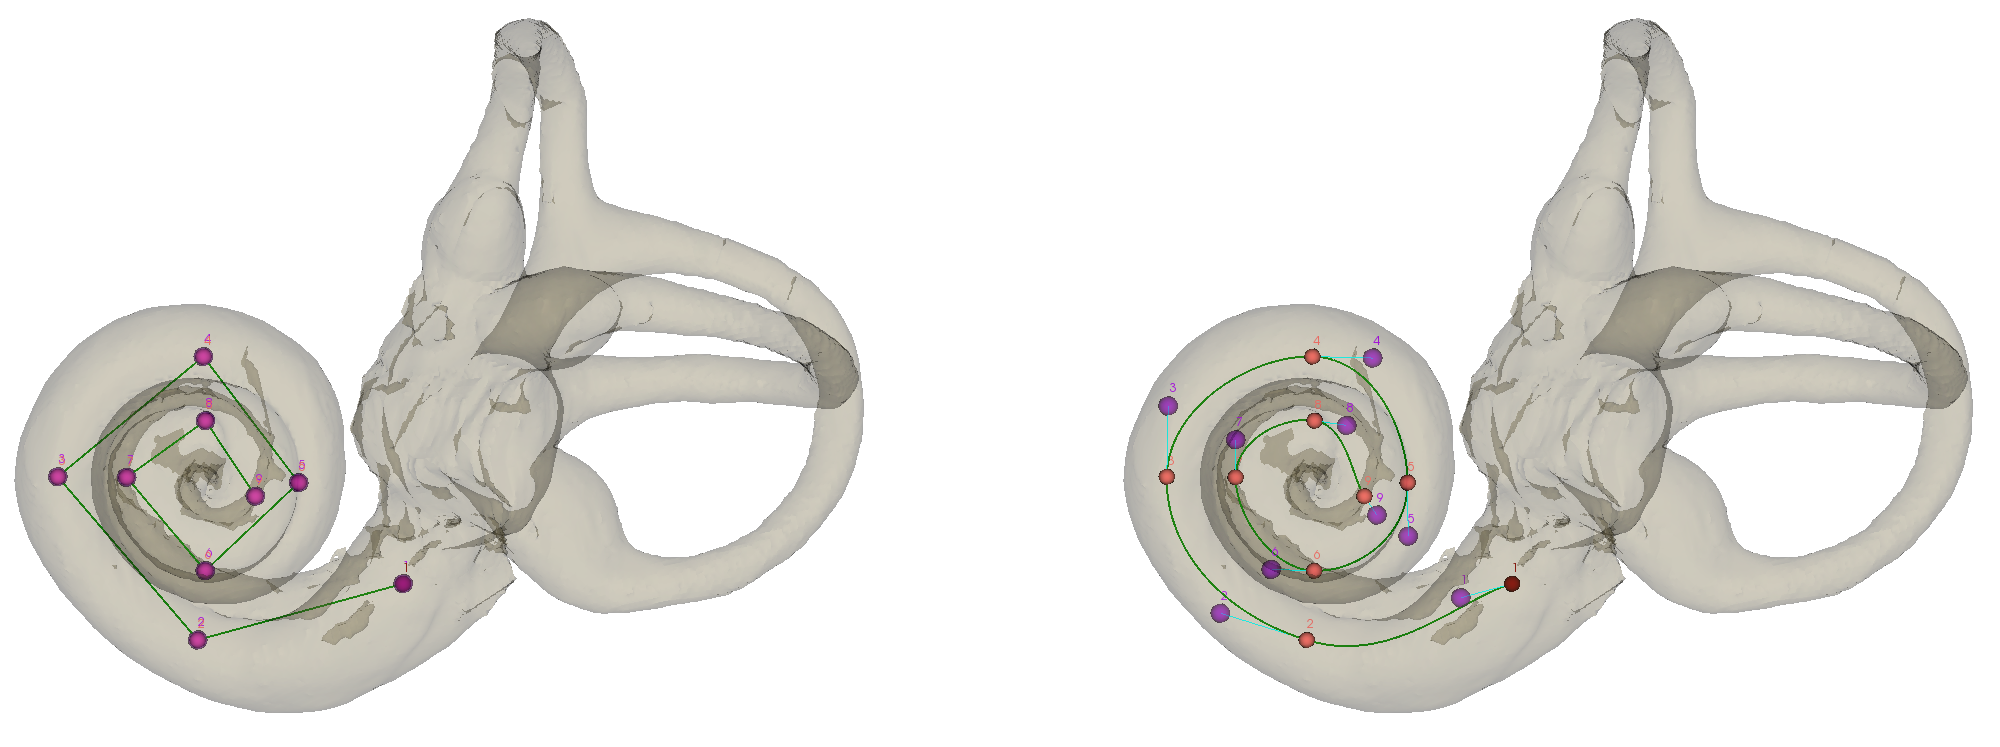
\includegraphics[scale=0.23]{images/10/move_selected_handles_input_output.png} 
	\caption{Example of curve handles semi-automatic displacement (movement intensity: 25\%).}
\label{move_handles2}
 
\end{figure}

\begin{figure}
  \centering
  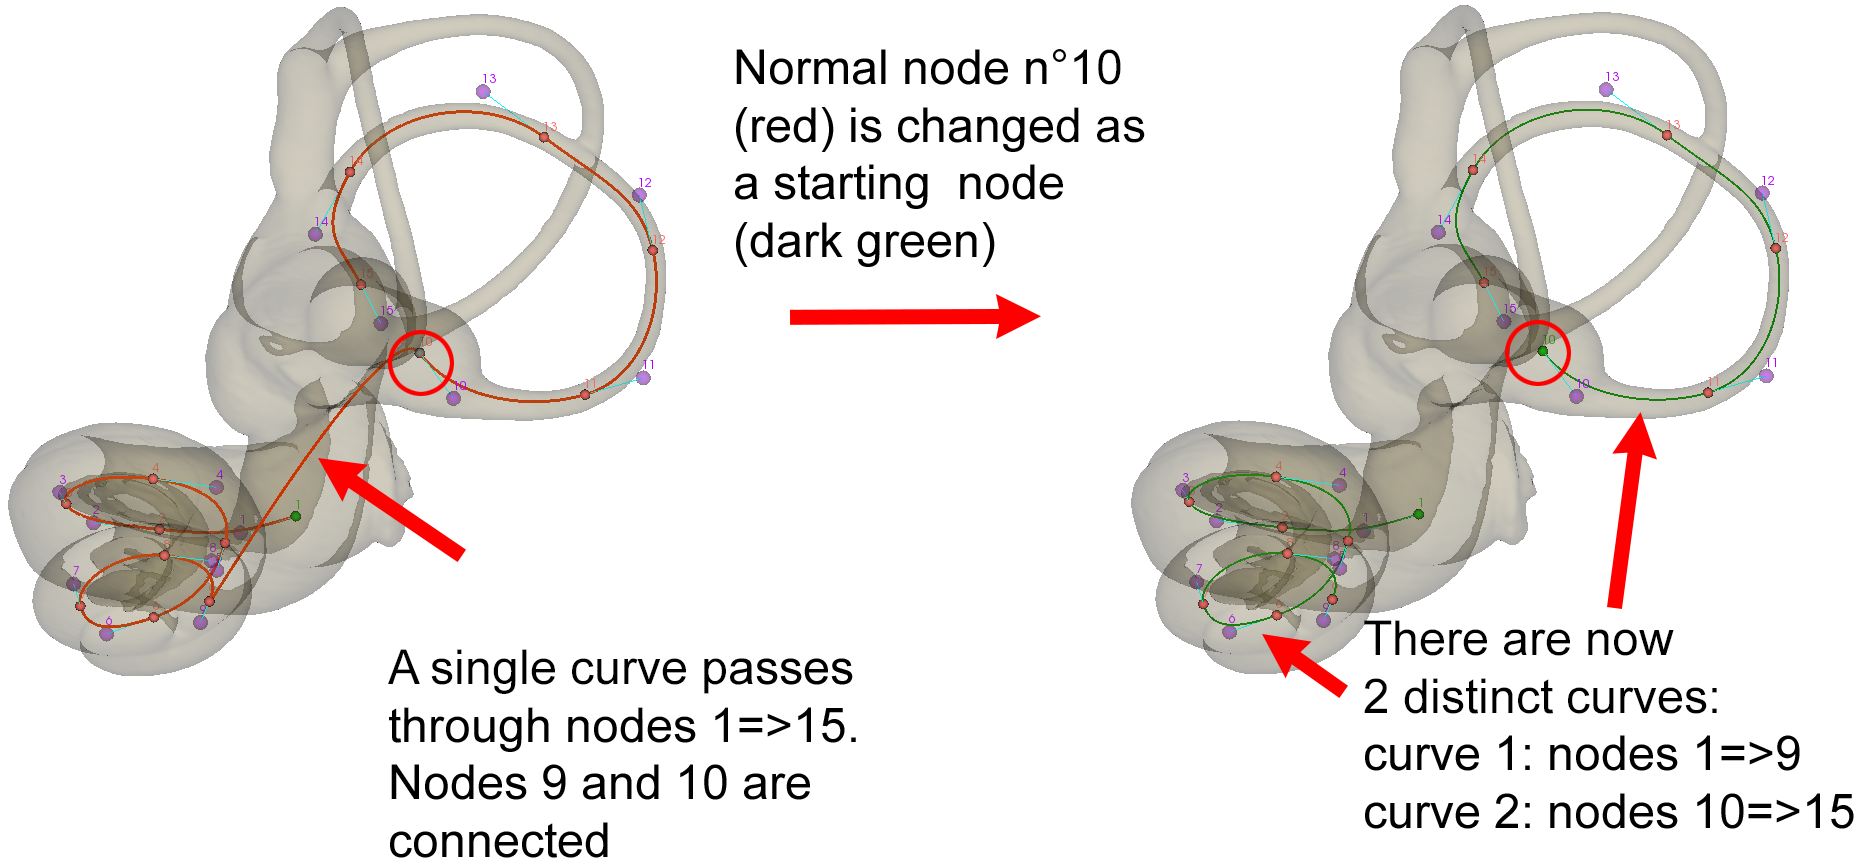
\includegraphics[scale=0.23]{images/10/change_node_as_curve_starting_point.png} 
	\caption{Curve decomposition into segments (left bony labyrinth of \textit{Galago moholi}). Left: a single curve passes through 15 curve node landmarks. Right: curve node n\degree10 was defined as a new curve starting point. Now, there are two curves. The first curve passes through the cochlea only (nodes 1 to 9). The second one passes through the lateral semicircular canal (nodes 10 to 15).}
\label{starting_node}
 
\end{figure}


\begin{figure}
  \centering
  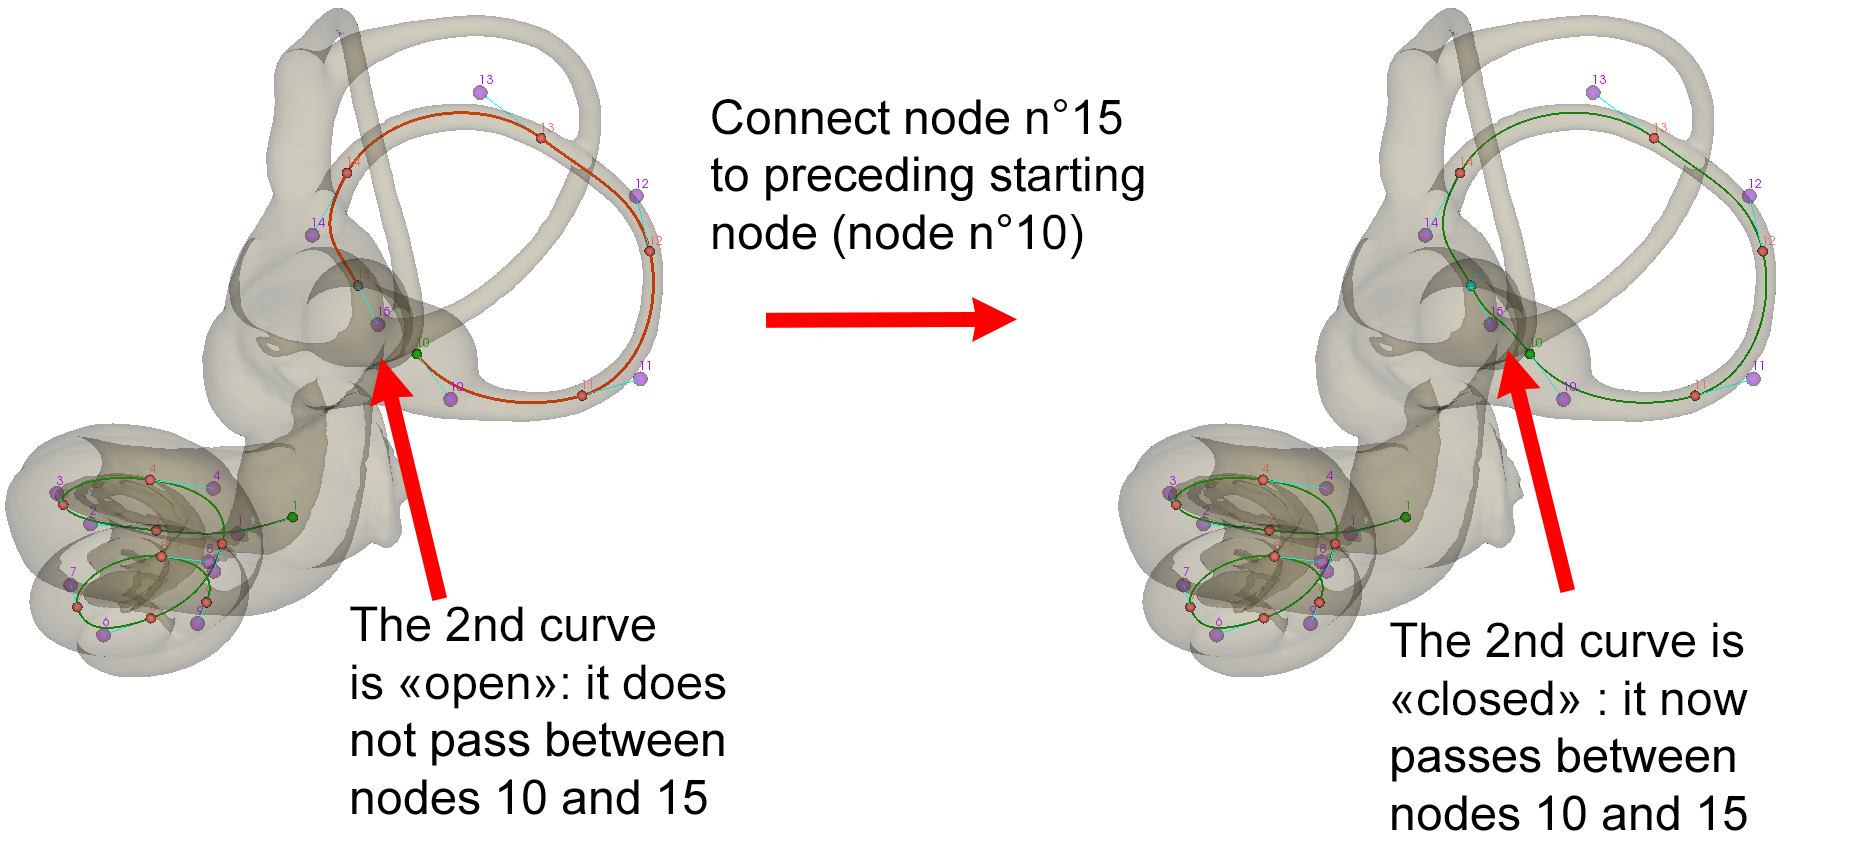
\includegraphics[scale=0.23]{images/10/connect_node_to_preceding_starting_point.png} 
	\caption{Closing curve segments (left bony labyrinth of \textit{Galago moholi}). Left: the curve segment passing through the lateral semicircular canal is "open": the curve does not pass through the first curve node (node n\degree10) and the last one (node n\degree15). Right: curve node n\degree15 was connected to the preceding curve starting node n\degree10. Now, the curve passing through the lateral semicircular canal is "closed".}
\label{connect_to_preceding_starting_node}
\end{figure}

\begin{figure}
  \centering
  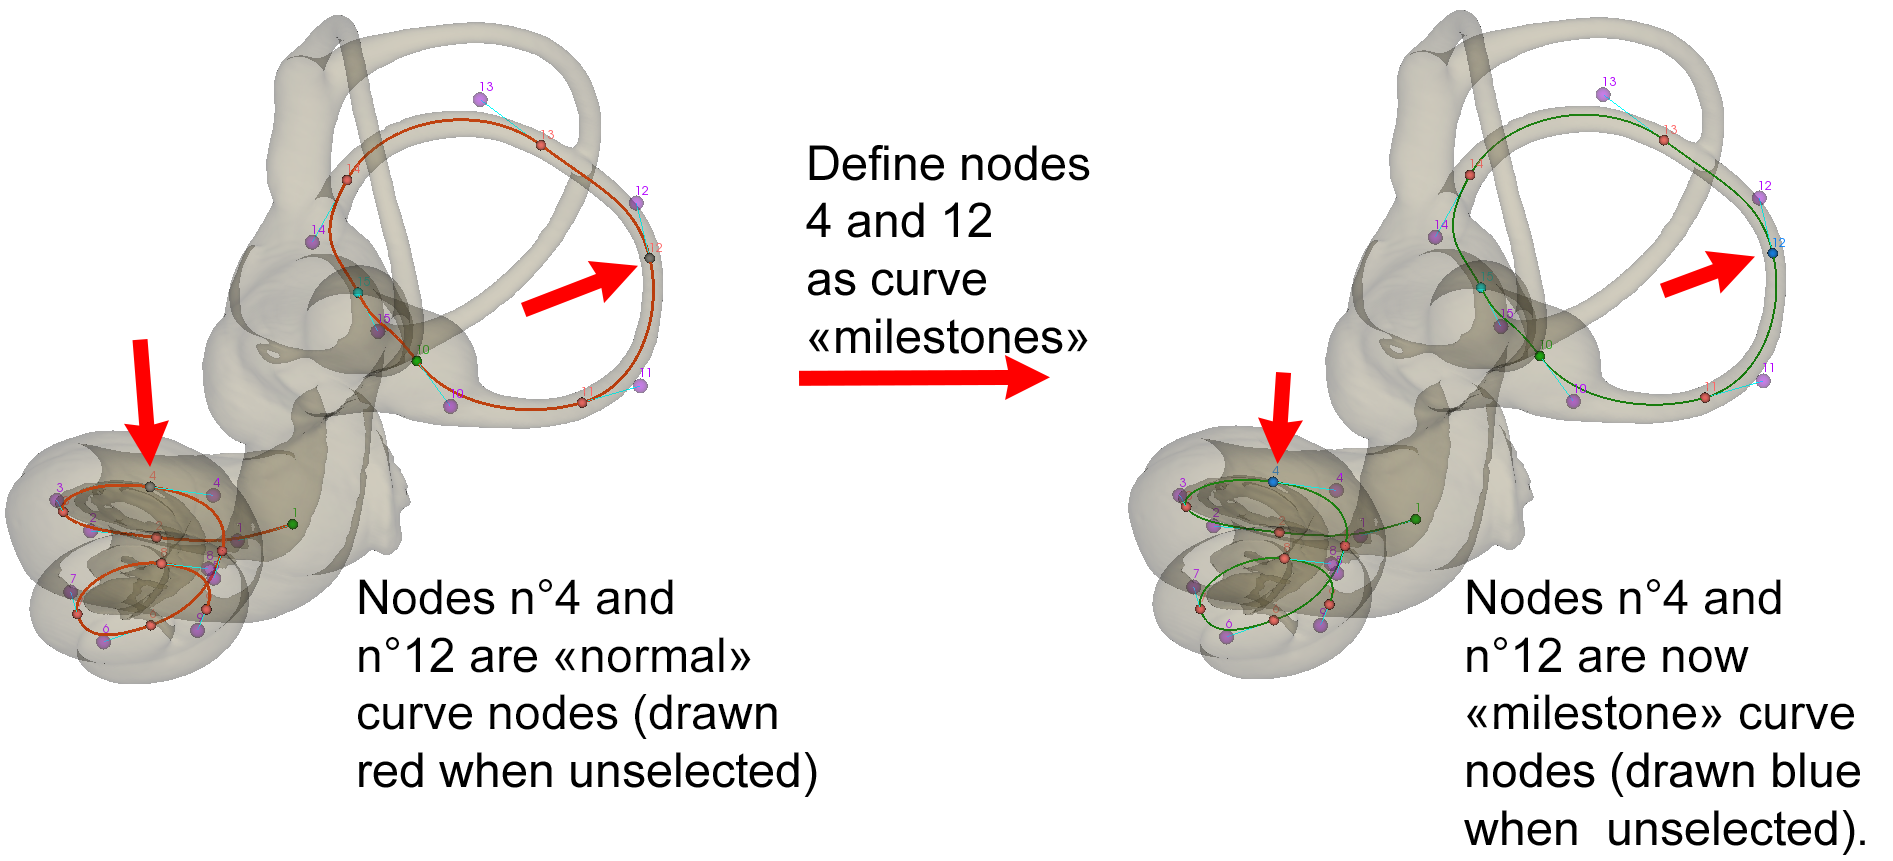
\includegraphics[scale=0.23]{images/10/curve_milestones.png} 
	\caption{Curve decomposition into \textbf{contiguous} segments (left bony labyrinth of \textit{Galago moholi}). Left: curve 1 (nodes 1-9) passes through the cochlea; curve 2 passes through the lateral semicircular canal (nodes 10-15). Right: curve nodes 4 and 12 were defined as curve milestones. When exporting curve infos or landmarks, MorphoDig now considers that 4 curve segments exist: curve 1 (nodes 1-4); curve 2 (nodes 4-9); curve 3 (nodes 10-12); curve 4 (nodes 12-15).}
\label{curve_milestone}
\end{figure}

\subsection{Normal nodes (red): change as starting modes (dark green)}\label{section_curve_segment1}
This option makes it possible to decompose a "long" curve passing through a given number of curve nodes into distinct \textbf{"independent"} curve segments. A practical example is shown in Fig. \ref{starting_node} p. \pageref{starting_node}. Selected node landmarks will be given flag ``1". Please also refer to section \ref{file_curve_section} p.\pageref{file_curve_section}.


\subsection{Normal nodes (red): connect to preceding starting nodes (cyan)}
This option makes it possible to "close" curve segments by connecting the last node of a curve segment to the starting point of that curve segment. A practical example is shown in Fig. \ref{connect_to_preceding_starting_node} p. \pageref{connect_to_preceding_starting_node}. Selected node landmarks will be given flag ``3". Please also refer to section \ref{file_curve_section} p.\pageref{file_curve_section}.



\subsection{Normal nodes (red): define as milestone (blue)}\label{section_curve_segment2}
This option makes it possible to decompose a curve passing through a given number of curve nodes into \textbf{"contiguous"} curve segments. A practical example is shown in Fig. \ref{curve_milestone} p. \pageref{curve_milestone}. Each curve milestone is involved into 2 curve segments: it acts as the ending node of a given curve, and as the starting point of the following curve. Curve milestones are given flag ``2".




\subsection{Reset selected nodes to Normal nodes (red)}
Special nodes (curve starting points, nodes connected to their preceding starting points, and curve milestones) are reset back to a "normal" state when using this option. Selected landmark are given flag ``0".

\noindent Further information regarding curve use in MorphoDig is available in the section ``File $\rightarrow$
Curves" section (section \ref{file_curve_section} p.\pageref{file_curve_section}) and in the tutorial ``working with curves".

\section{Edit color of all selected flag landmarks}
\noindent
\begin{minipage}{0.5\textwidth}
Using this option, you can modify the color of all selected flag landmarks at once.
\end{minipage}    
\begin{minipage}{0.5\textwidth}\centering
  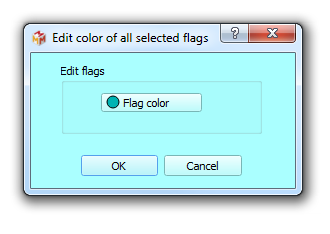
\includegraphics[scale=0.5]{images/10/edit_color_all_selected_flags.png}
 \captionof{figure}{Edit color of all selected flags dialog}
 \end{minipage} 


\section{Edit length of all selected flag landmarks}
\noindent
\begin{minipage}{0.5\textwidth}
Using this option, you can modify the length of all selected flag landmarks at once.
\end{minipage}    
\begin{minipage}{0.5\textwidth}\centering
  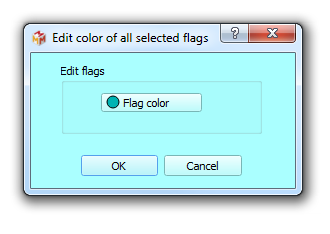
\includegraphics[scale=0.5]{images/10/edit_color_all_selected_flags.png}
 \captionof{figure}{Edit length of all selected flags dialog}
 \end{minipage} 




\section{Update all selected flag landmarks' color to that of the closest vertex}

This option will set the color of all selected flag landmarks to that of the closest vertex found in all opened surface objects. A practical example is shown in Fig. \ref{flag_color_closest_vertex} p. \pageref{flag_color_closest_vertex}.

\begin{figure}
  \centering
  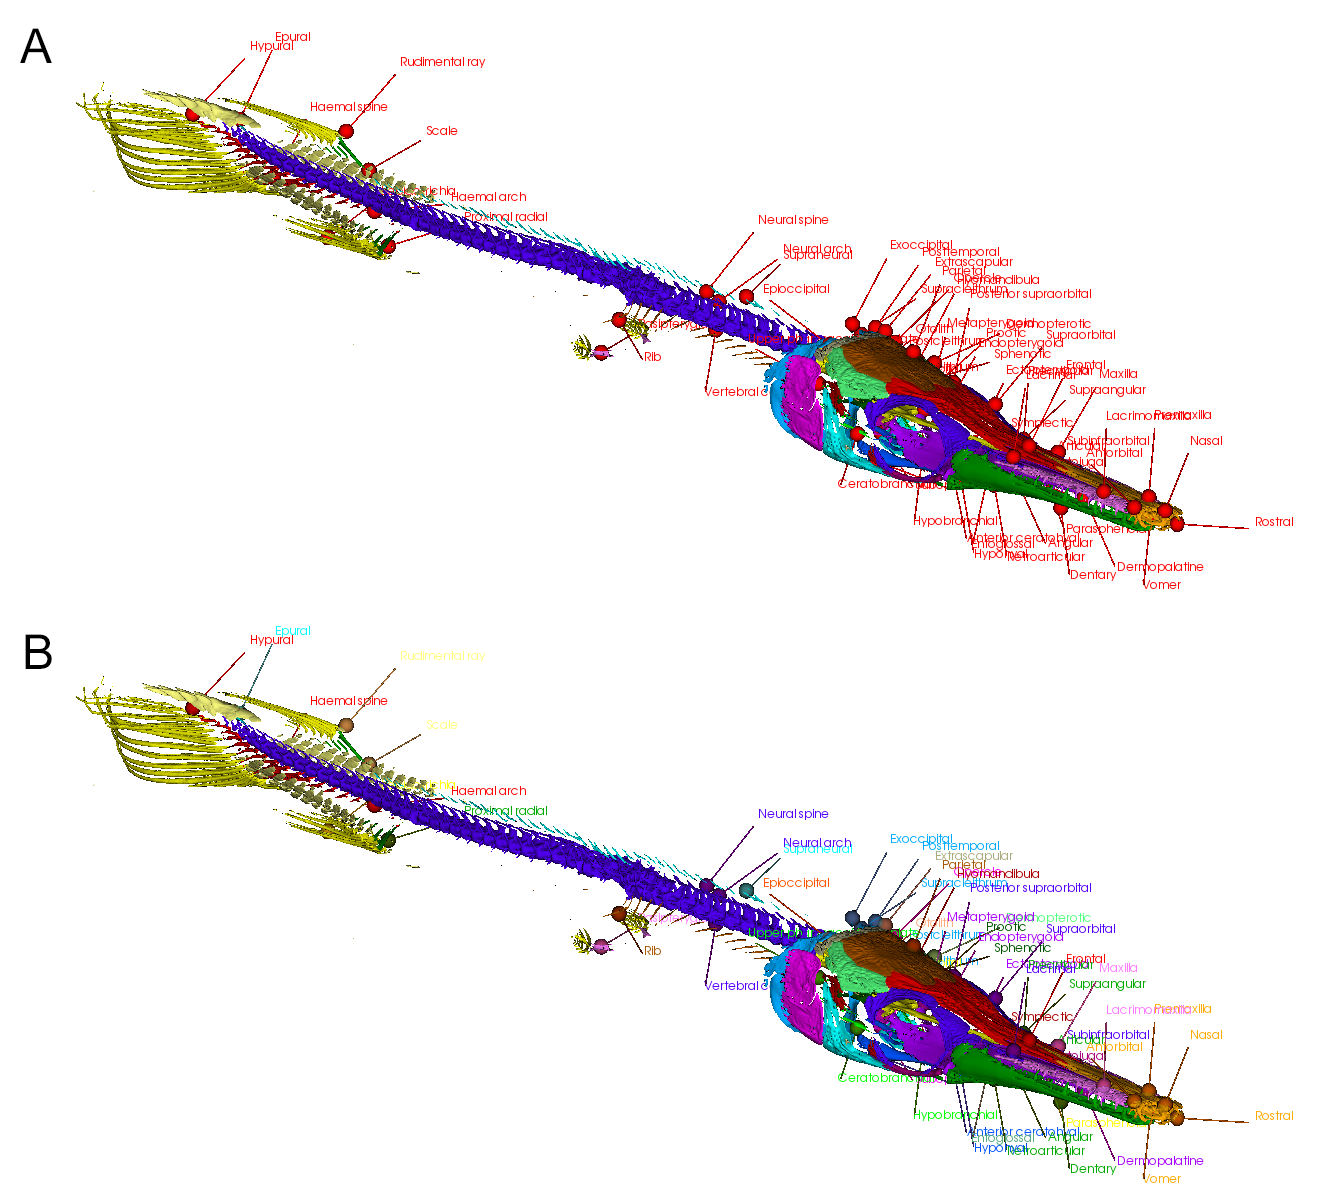
\includegraphics[scale=0.31]{images/10/edit_flag_color_closest_vertex.png} 
	\caption{Setting the color for all flags according to the closest vertices' color of a tagged 3D model of skeletton of \textit{Atractosteus tristoechus}. A: the flags are initially all  drawn in red. B: all flags are now given colors that correspond to that of the closest vertices found for each flag.}
\label{flag_color_closest_vertex}
\end{figure}
